\documentclass{article}
\usepackage{amsmath}
\usepackage{hyperref}
\usepackage{graphicx}
\usepackage{minted}
\usepackage{siunitx}
\usepackage[UTF8]{ctex}

\hypersetup{
  colorlinks=true,
  allcolors=blue,
  pdfstartview=Fit,
  breaklinks=true
}

\begin{document}
  \title{系统开发工具基础 \\ 第二周实验报告}
  \author{乔海轩—25090012035}
  \date{2026年8月31日}
  \maketitle
  
  \tableofcontents
  \newpage

  \section{总览}
    \begin{table}[h]
      \centering
      \begin{tabular}{|l|l|c|}
        \hline
        题目编号 & 描述 & 完成情况 \\
        \hline
        5 & 控制一个可清理的后台任务 & 已完成 \\
        6 & 语义重构与本地开发反馈 & 已完成 \\
        7 & 用调试器定位归并排序缺陷 & 已完成 \\
        8 & 先测量，再优化慢速词频程序 & 已完成 \\
        \hline
      \end{tabular}  
    \end{table}
    Github 仓库地址：\href{https://github.com/Ptilotsis-o/system-dev-tools/}{https://github.com/Ptilotsis-o/system-dev-tools/}
    \newline Commit记录如图\ref{fig:commit}所示。
    \begin{figure}[h]
      \centering
      
\includegraphics[width=0.8\textwidth]{figures/commit.png}
      \caption{Commit记录截图}
      \label{fig:commit}
    \end{figure}
  
  \newpage
  \section{第 5 题 控制一个可清理的后台任务}
    \subsection*{题目要求}
      \begin{itemize}
        \item 赋予脚本执行权限，在前台启动，并把 stdout、stderr 分别写入 stdout.log、stderr.log。
        \item 使用 \texttt{Ctrl-Z} 挂起任务，再用 \texttt{bg} 让它在后台继续；使用 \texttt{jobs} 确认状态。
        \item 使用 \texttt{jobs -p} 或等价方式取得 PID，不得手工抄写 PID；发送 \texttt{SIGTERM} 并等待任务结束。
        \item 确认 \texttt{cleanup.log} 中出现 \texttt{CLEAN\_EXIT}，且任务已经退出；禁止使用 kill -9。
      \end{itemize}
    \subsection*{操作步骤与命令}
      \begin{minted}{bash}
        chmod +x worker.sh
        ./worker.sh > stdout.log 2> stderr.log
        Ctrl-Z
        bg
        jobs
        pid=$(jobs -p)
        kill $pid
        jobs
        cat cleanup.log
      \end{minted}
    \subsection*{结果验证}
      \begin{itemize}
        \item \texttt{stdout.log} 和 \texttt{stderr.log} 为空（符合预期）；
        \item \texttt{cleanup.log} 内容为 \texttt{CLEAN\_EXIT}；
        \item 执行 \texttt{kill} 后，\texttt{jobs} 不再显示该任务，进程正常退出；
        \item 未使用 \texttt{kill -9}，证明进程捕获了 \texttt{SIGTERM} 并执行了清理。
      \end{itemize}
      \begin{figure}[h]
        \centering
        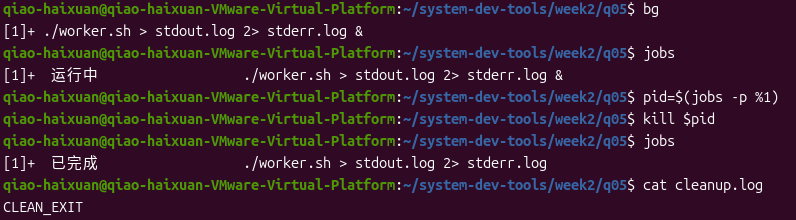
\includegraphics[width=0.8\textwidth]{figures/jobs.png}
        \caption{部分指令截图}
        \label{fig:jobs}
      \end{figure}
  
  \newpage
  \section{第 6 题 语义重构与本地开发反馈}
    \subsection*{题目要求}
      \begin{itemize}
        \item 在已配置好 Python、pytest 和 ruff 的课程环境中打开 q06，并启用 Python 语言服务器。
        \item 分别演示跳转到定义和查找引用。
        \item 使用“重命名符号”把 \texttt{total\_price} 改为 \texttt{calculate\_total}，保证定义和所有代码引用同步改变。
        \item 在 \texttt{app.py} 中临时加入未使用的 \texttt{import os}，用 \texttt{ruff check} 发现并删除；最后运行 \texttt{ruff check} 和 \texttt{pytest} 并保证通过。
      \end{itemize}
    \subsection*{操作步骤与命令}
      \begin{minted}{bash}
        source venv/bin/activate
        vim app.py
        # 完成gd 、gf、重命名等操作
        vim app.py # 临时加入 import os
        ruff check
        vim app.py # 删除 import os
        ruff check
        pytest
      \end{minted}
    \subsection*{结果验证}
      \begin{itemize}
        \item \texttt{gd} 能够跳转到定义 \texttt{total\_price} 定义，\texttt{gf} 能够跳转到 \texttt{total\_price} 引用位置；
        \item \texttt{ \textbackslash rn} 将 \texttt{total\_price} 重命名为 \texttt{calculate\_total}；
        \item \texttt{ruff} 不报错，\texttt{pytest} 通过。
      \end{itemize}
      \begin{figure}[h]
        \centering
        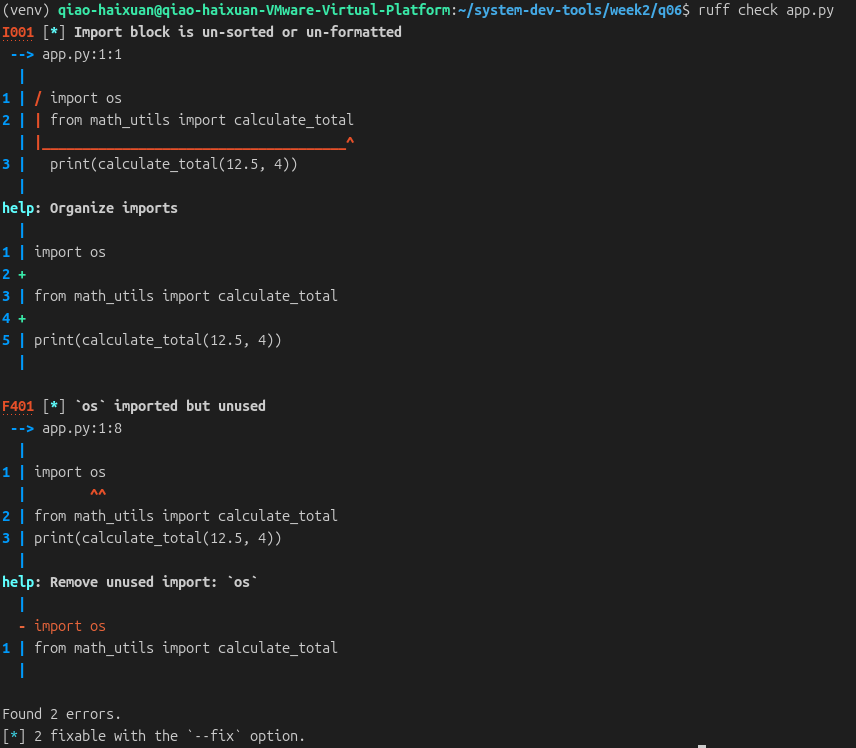
\includegraphics[width=0.8\textwidth]{figures/ruff.png}
        \caption{ruff报错时截图}
        \label{fig:ruff}
      \end{figure}
      \begin{figure}[h]
        \centering
        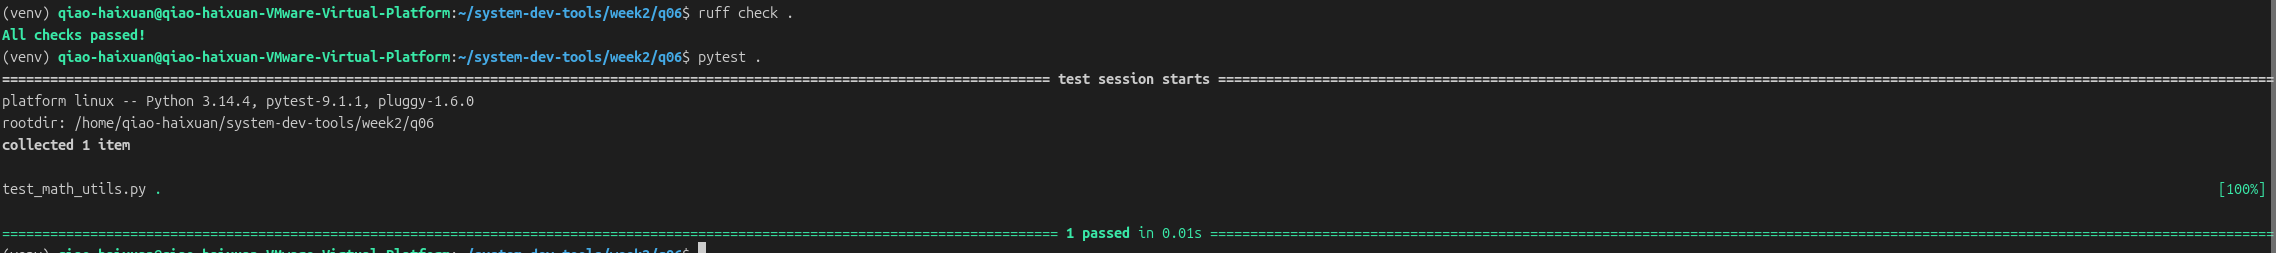
\includegraphics[width=0.8\textwidth]{figures/ruffpytest.png}
        \caption{ruff和pytest检查截图}
        \label{fig:ruff_and_pytest_check}
      \end{figure}
   
  \newpage    
  \section{第 7 题 用调试器定位归并排序缺陷}
    \subsection*{题目要求}
      \begin{itemize}
        \item 先运行给定输入，确认结果错误或出现异常。
        \item 使用 pdb、IDE debugger 或等价调试器，在 merge 中设置断点并观察 i、j、left[i]、right[j]。
        \item 完成最小修复，不得用 sorted 替换归并排序。
        \item 使用 pytest 增加两个测试：给定输入和含重复元素的列表；保证测试通过。
      \end{itemize}
    \subsection*{操作步骤与命令}
      \begin{minted}{bash}
        python merge_sort.py
        vim merge_sort.py
        python merge_sort.py
        # 调试指令，此处略
        vim merge_sort.py
        vim test_merge_sort.py
        pytest
      \end{minted}
    \subsection*{结果验证}
      \begin{itemize}
        \item 初次运行\texttt{merge\_sort.py}，结果错误。
        \item 为\texttt{merge\_sort.py} 添加断点，使用 \texttt{pdb}，观察 i、j、left[i]、right[j]。
        \item 修复\texttt{merge\_sort.py} 中的错误，确保归并排序正确。
        \item 编写测试用例，运行\texttt{pytest}，确认测试通过。
      \end{itemize}
      \begin{figure}[h]
        \centering
        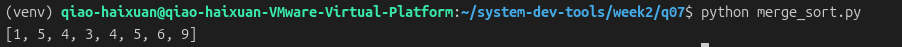
\includegraphics[width=0.8\textwidth]{figures/wrongresult.png}
        \caption{初次运行时的错误结果}
        \label{fig:wrongresult}
      \end{figure}
      \begin{figure}[h]
        \centering
        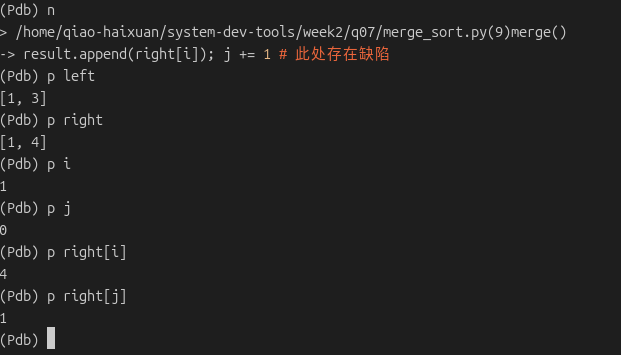
\includegraphics[width=0.8\textwidth]{figures/pdb.png}
        \caption{pdb发现逻辑错误时的截图}
        \label{fig:pdb}
      \end{figure}
      \begin{figure}[h]
        \centering
        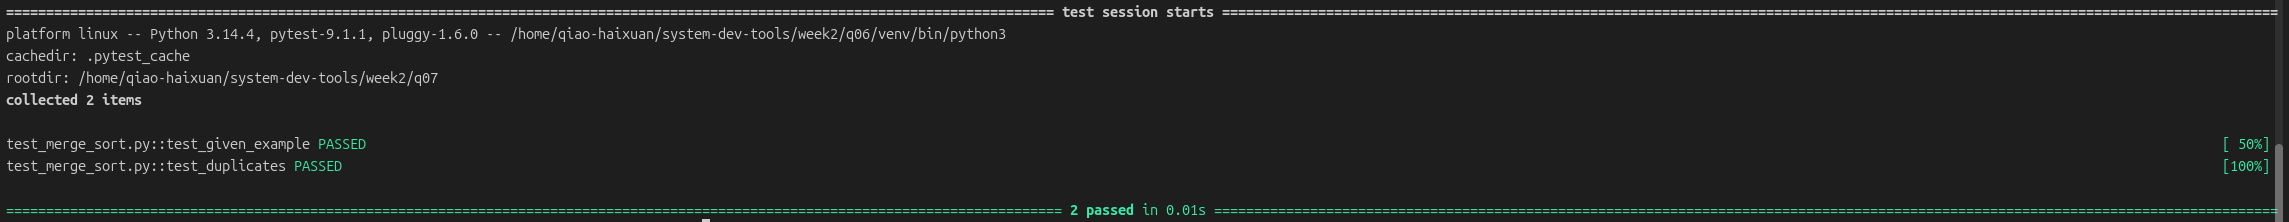
\includegraphics[width=0.8\textwidth]{figures/pytest.png}
        \caption{pytest输出截图}
        \label{fig:pytest}
      \end{figure}
  
  \newpage
  \section{第 8 题 先测量，再优化慢速词频程序}
    \subsection*{题目要求}
      \begin{itemize}
        \item 生成 \texttt{words.txt} 文件，使用 \texttt{time} 运行原程序 2 次并记录耗时。
        \item 使用 \texttt{cProfile -s cumulative} 运行一次，找出主要耗时位置。
        \item 在不改变最终 count 的前提下优化程序；不得写死 1000。
        \item 使用相同输入再运行 2 次，计算优化前后中位数和加速比。
      \end{itemize}
      \subsection*{操作步骤与命令}
        \begin{minted}{bash}
          python generate_words.py
          time python word_freq.py
          time python word_freq.py
          cProfile -s cumulative word_freq.py
          vim word_freq.py
          time python word_freq.py
          time python word_freq.py
        \end{minted}
      \subsection*{结果验证}
        \begin{itemize}
          \item 生成了 \texttt{words.txt} 文件。
          \item 运行原程序和优化后的程序各 2 次，记录耗时，\texttt{cProfile -s cumulative} 输出主要耗时位置。
          \item 优化前中位数为 \SI{0.1685}{\second} ，优化后中位数为 \SI{0.0315}{\second} ，加速比为 \SI{81.3}{\%} 。
        \end{itemize}
        \begin{figure}[h]
          \centering
          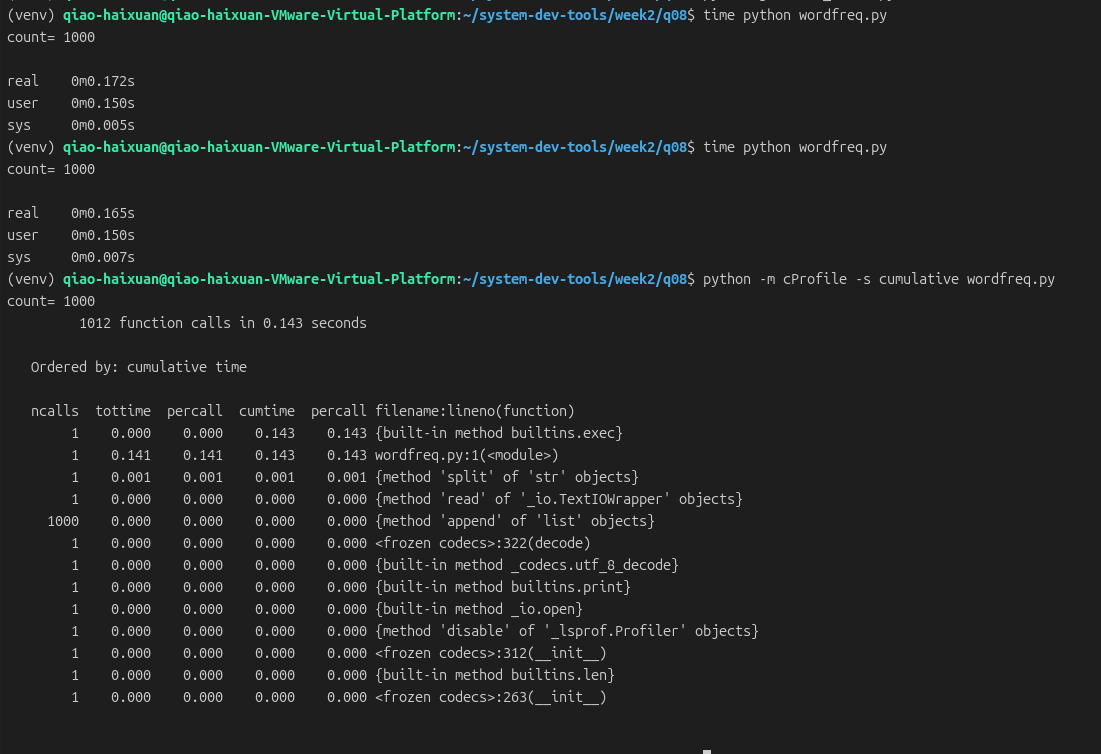
\includegraphics[width=0.8\textwidth]{figures/cProfile.png}
          \caption{优化前 time 和 cProfile 输出截图}
          \label{fig:cProfile}
        \end{figure}
        \begin{figure}[h]
          \centering
          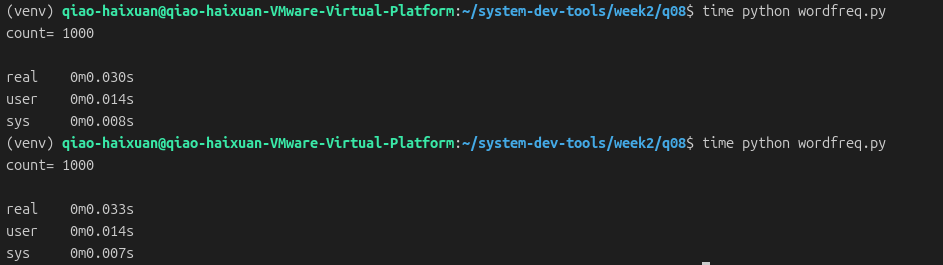
\includegraphics[width=0.8\textwidth]{figures/time.png}
          \caption{ 优化后 time 截图}
          \label{fig:time}
        \end{figure}

  \newpage
  \section{课后作业}
    \subsection{q1: 捕获自定义信号 SIGUSR1}
    目标：创建 \texttt{sig\_demo.sh}，使用 \texttt{trap} 捕获 \texttt{SIGUSR1}，收到信号时向 \texttt{usr1.log} 写入 \texttt{"USR1 received"}。在后台启动脚本，通过 \texttt{kill -USR1 <pid>} 发送信号，验证日志内容。
      \begin{minted}{bash}
        chmod +x sig_demo.sh
        ./sig_demo.sh &
        pid=$! 
        kill -USR1 $pid
        cat usr1.log
        kill $pid
      \end{minted}
      \begin{figure}[h]
        \centering
        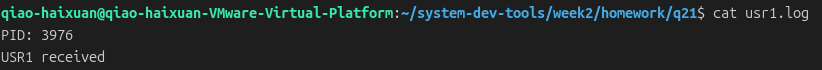
\includegraphics[width=0.8\textwidth]{figures/kill.png}
        \caption{kill -USR1 <pid> 发送信号，验证日志内容}
        \label{fig:kill}
      \end{figure}
    \subsection{q2: 前后台切换练习}
    目标：启动 \texttt{ping 127.0.0.1 > ping.log}，使用 \texttt{Ctrl-Z} 挂起，再用 \texttt{bg} 放到后台，然后用 \texttt{fg} 调回前台，最后用 \texttt{Ctrl-C} 终止。记录每一步的 \texttt{jobs} 输出。
      \begin{minted}{bash}
        ping 127.0.0.1 > ping.log &
        Ctrl-Z
        jobs
        bg
        jobs
        fg
        ctrl-c
      \end{minted}
      \begin{figure}[h]
        \centering
        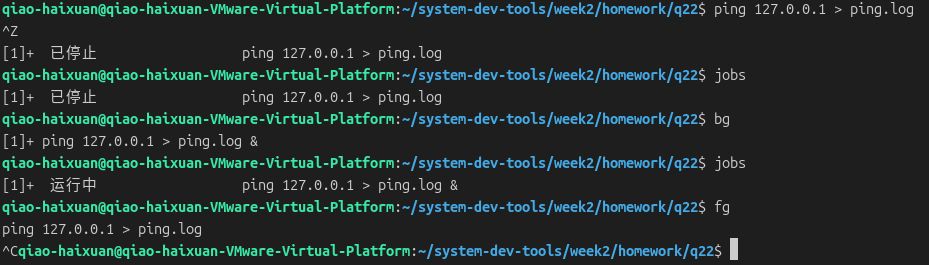
\includegraphics[width=0.8\textwidth]{figures/ping.png}
        \caption{ping 127.0.0.1 > ping.log \& 挂起、放到后台、调回前台、终止，记录 jobs 输出}
        \label{fig:ping}
      \end{figure}
    \subsection{q3: 多任务控制}
    目标：同时启动两个脚本 \texttt{w1.sh}（无限输出 A）和 \texttt{w2.sh}（无限输出 B），将 stdout 分别重定向到 \texttt{a.log} 和 \texttt{b.log}。用 \texttt{jobs} 查看状态，并用 \texttt{kill \%1 \%2} 同时终止两个任务。
      \begin{minted}{bash}
        chmod +x w1.sh
        chmod +x w2.sh
        ./w1.sh > a.log &
        ./w2.sh > b.log &
        jobs
        kill %1 %2
      \end{minted}
      \begin{figure}[h]
        \centering
        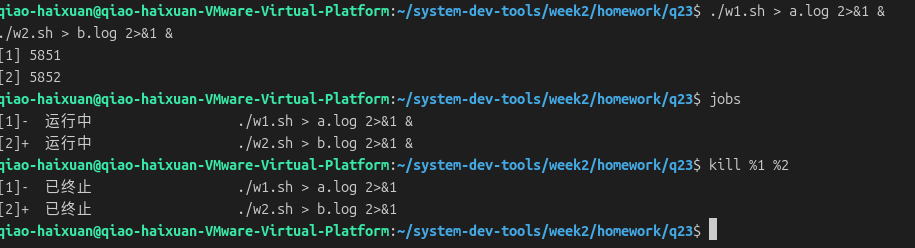
\includegraphics[width=0.8\textwidth]{figures/jobs_2.png}
        \caption{jobs 输出截图，终止两个任务后为空}
        \label{fig:jobs_2}
      \end{figure}
    \subsection{q4: 使用 wait 等待后台任务}
    目标：编写脚本，后台启动 \texttt{sleep 5}，使用 \texttt{wait} 等待其结束，结束后输出 \texttt{"Done"} 到 \texttt{wait.log}。用 \texttt{time} 测量整体耗时，确认等待生效。
      \begin{minted}{bash}
        time bash wait_demo.sh
        cat wait.log
      \end{minted}
      \begin{figure}[h]
        \centering
        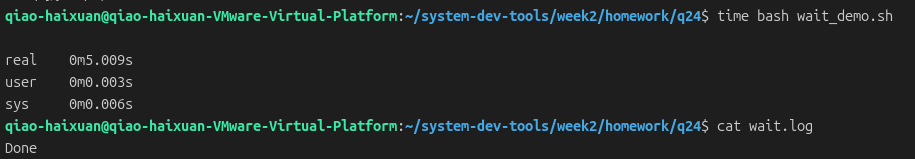
\includegraphics[width=0.8\textwidth]{figures/wait.png}
        \caption{wait.log 输出截图}
        \label{fig:wait}
      \end{figure}
    \subsection{q5: 重命名类名 Person→User}
    目标：创建 \texttt{person.py} 定义类 \texttt{Person}，在 \texttt{main.py} 中实例化并调用。使用语言服务器的“重命名符号”功能将 \texttt{Person} 改为 \texttt{User}，确保所有引用同步更新，并运行验证。
      将光标移至\texttt{person.py} 中的 \texttt{Person} 类名，通过\texttt{\textbackslash{} rn} 重命名，修改为\texttt{User}。
    \subsection{q6: 查找引用与跳转}
    目标：在 \texttt{const.py} 中定义常量 \texttt{PI = 3.14159}，并在 \texttt{area.py}、\texttt{volume.py} 中导入使用。使用“查找所有引用”列出所有使用 \texttt{PI} 的位置，并用“跳转到定义”确认来源。
      将光标移至\texttt{const.py} 中的 \texttt{PI} 定义，通过\texttt{gr}查找所有引用。
    \subsection{q7: 使用 ruff 修复格式问题}
    目标：创建格式混乱的 \texttt{messy.py}（含多余空格、缺少空行、行尾空白等）。运行 \texttt{ruff check --fix} 自动修复，再运行 \texttt{ruff format} 统一格式，确保无报错。
      \begin{minted}{bash}
        ruff check --fix messy.py
        ruff format messy.py
        ruff check messy.py
      \end{minted}
    \subsection{q8: 调试递归斐波那契的边界条件}
    目标：提供有缺陷的 \texttt{fib} 函数（当 \texttt{n=0} 时返回 1）。使用调试器单步跟踪 \texttt{fib(0)} 的调用过程，定位错误并修复，然后编写 \texttt{pytest} 测试验证 \texttt{fib(0)==0}、\texttt{fib(1)==1}、\texttt{fib(5)==5}。
      \begin{minted}{bash}
        vim fib_bug.py
        pytest test_fib.py
      \end{minted}
      \begin{figure}[h]
        \centering
        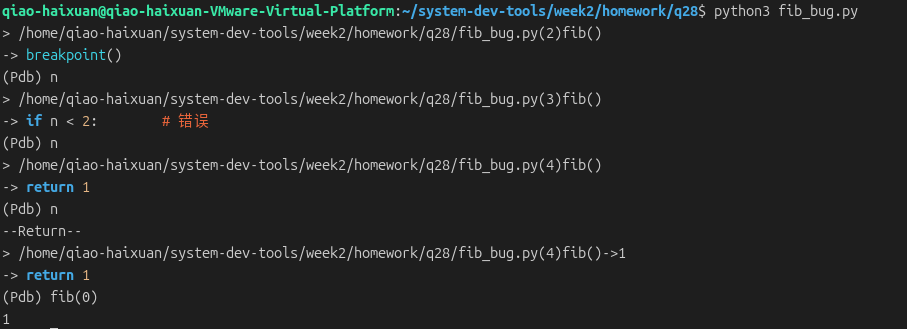
\includegraphics[width=0.8\textwidth]{figures/debug.png}
        \caption{fib\_bug.py 调试截图}
        \label{fig:debug}
      \end{figure}
      \begin{figure}[h]
        \centering
        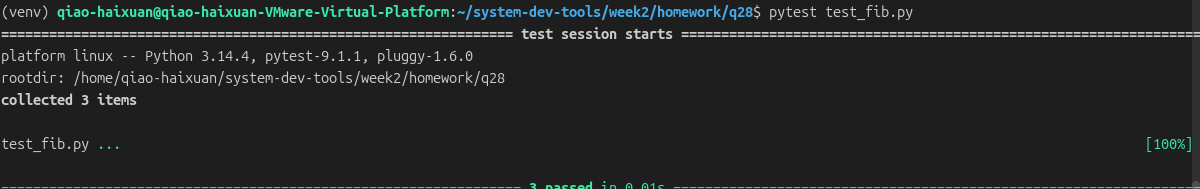
\includegraphics[width=0.8\textwidth]{figures/test.png}
        \caption{pytest test\_fib.py 输出截图}
        \label{fig:test}
      \end{figure}
    \subsection{q9: 调试列表插入的越界}
    目标：供 \texttt{safe\_insert} 函数，当索引越界时抛出 \texttt{IndexError}。调用 \texttt{safe\_insert([1,2,3], 5, 99)} 触发异常，使用调试器观察 \texttt{idx} 与 \texttt{len(arr)}，修复逻辑（如越界时追加到末尾），并添加测试。
      \begin{minted}{bash}
        vim safe_insert.py
        pytest test_safe_insert.py
      \end{minted}
      \begin{figure}[h]
        \centering
        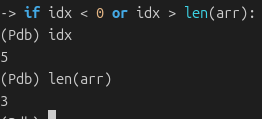
\includegraphics[width=0.8\textwidth]{figures/debug2.png}
        \caption{safe\_insert.py 调试截图}
        \label{fig:debug}
      \end{figure}
      \begin{figure}[h]
        \centering
        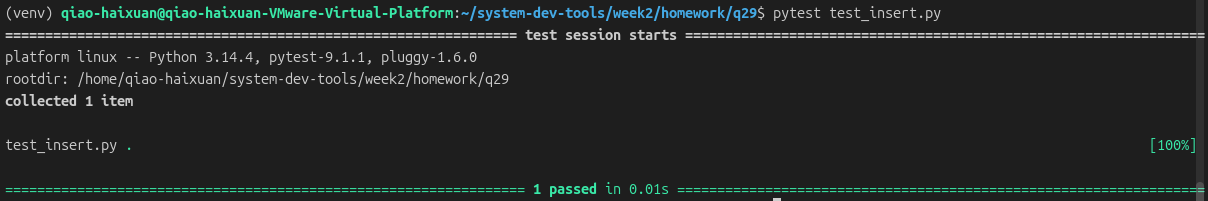
\includegraphics[width=0.8\textwidth]{figures/test2.png}
        \caption{pytest test\_safe\_insert.py 输出截图}
        \label{fig:test2}
      \end{figure}
    \subsection{q10: 分析正则表达式重复编译的瓶颈}
    目标：创建 \texttt{regex\_slow.py}，在循环内部反复调用 \texttt{re.compile}。使用 \texttt{cProfile} 定位 \texttt{re.\_compile} 热点，将编译提到循环外进行预编译优化，测量前后耗时并计算加速比。
      \begin{minted}{bash}
        time python regex_slow.py
        time python regex_slow.py
        python -m cProfile -s cumulative regex_slow.py
        time python regex_fast.py
        time python regex_fast.py
      \end{minted}
      优化前时间中位数为0.020秒，优化后中位数为0.016秒。
    \subsection{课后作业commit记录}
      \begin{figure}[h]
        \centering
        
\includegraphics[width=0.8\textwidth]{figures/homework_commit.png}
        \caption{课后作业commit记录}
        \label{fig:homework_commit}
      \end{figure}
    
  \section{解题感悟}
    本次实验报告涵盖了系统开发工具基础的进程管理、代码重构、调试与性能优化等方面。通过实际操作，我掌握了信号捕获、前后台任务切换、语言服务器重命名、pdb调试以及使用 time 和 cProfile 定位瓶颈。课后作业进一步巩固了这些技能，尤其是在处理自定义信号、正则预编译优化等问题时，提升了分析与解决问题的能力。总的来说，这次实验让我对命令行环境和开发工具有了更深入的理解，为后续工程实践打下了基础。

\end{document}